\section{Usage examples}

In this section, we will give a few example programs written in the
DSL, to give a flair for the kind of scene description language that
emerged from our design choices.

There were different types of sounds specified by game masters and sound designers, based on the planned usage and design requirements of the sound. There were ambient sound loops used to simulate states such as running the ships main reactor or the sounds of massive computer banks running in the sensor processing room. There were feedback sounds triggered in response to participant actions, such as loading a torpedo or triggering a sensor sweep. These sounds mainly functioned as both confirmation to the participant that the system has registered the event and to communicate the occurrence of an event to participants in other parts of the ship. Apart from these sounds, the game masters had access to a wide variety of sounds and noises with no predetermined meaning in order to simulate everything from debris hitting the outer hull to onboard fighting, as well as pre-recorded prologues used to segue players into the game at the start of each game session.

Some sounds needed to run through an Attack-Decay-Sustain-Release sequence, composed of multiple sound files and an arbitrarily long sustain-phase. Other sounds needed to trigger with fixed time intervals.

All sounds needed to be played on a set of speakers -- but not all sounds were to be played on all speakers when played. For example, sounds of airlock doors opening were played in the section containing the doors and sections immediately adjacent to it.

We built a setup script to handle all the sound setup in a repeatable and restartable way. The script had a \texttt{main} consisting of:
\begin{verbatim}
main = mapM_ (putStrLn . show) $ <soundlist>
\end{verbatim}
where the list of sounds was constructed in bits and pieces. We will explain and give examples for each section
of the sound list here.

We also defined and used a
single value for simultaneously addressing all sound sites (except the engine room
sub-woofer)
\begin{verbatim}
global = [1..11] :: [Segment] 
\end{verbatim}
as well as a utility command to help string together sound
declarations using the \texttt{SoundSpec} level concatenation
operator:
\begin{verbatim}
concatSS = foldl (:+) NopS
\end{verbatim}

\subsection{Noises and game start sounds}
\label{sec:noises}

The very easiest sounds to program for our DSL were the sounds that just needed to sound somewhere once. These consisted of a single sound file which was run all the way through.

All of these sounds were global. A typical sound definition for an
environmental noise would look like the noise of a distant explosion.

\begin{listing}
\begin{verbatim}
 Trigger "explosion distant 5" 
  (MatchEvent "sound.trigger.explosion.distant.5") 
  (Execute "explo distant 5" 
   (concatSS 
    (map 
     (\i -> Play "Random/explosions/explo_distant_med_05" i 0 (100,100))
     global)))
\end{verbatim}
\caption{Reactive event definition to play the sound of a distant explosion.}
\end{listing}
This sound would be triggered by the game masters by pushing a button in their sound control console that generated a \texttt{sound.trigger.explosion.distant.5} event on the joint \texttt{AMQP} communication bus.

The four different game starting sound sequences -- with mood-setting music and a spoken recap -- were triggered in the same way.

\begin{listing}
\begin{verbatim}
 Trigger "celestra act 3 trigger" 
  (MatchEvent "sound.trigger.act3") 
  (Execute "celestra act3" 
   (concatSS 
    (map 
     (\i -> Play "Story/Celestra_Akt3" i 0 (100,100)) 
     global)))
\end{verbatim}
\caption{Reactive event definition to start the game session starting
  sound sequences.}
\end{listing}

The same structure was used for game end sequences: depending on which of the six pre-written game ending sounds was deemed appropriate, a different trigger was sent over \texttt{AMQP}. This then phased over to an improvised game master epilogue spoken over the ship's PA system.

\subsection{Participant-triggered noises}
\label{sec:part-trigg-nois}

Several of the participant actions were supposed to trigger noises as well. Whenever one of the players initiated a sensor scan or a torpedo loading procedure, sounds were triggered that corresponded to that soundscape. The only fundamental difference between these and the game-mastering sounds described above was that the triggers used were game system events. As an example, we can consider the active scanning sensor system.

\begin{listing}
\begin{verbatim}
 Trigger "dradispingtrigger" 
  (MatchEvent "space.sensor.dradis.ping") 
  (Execute "dradisping" 
   (concatSS 
    (map 
     (\i -> Play "112_active_dradis" i 1000 (80,80) :+ 
            Play "330_activating_dradis" i 0 (100,100)) 
     global))),
\end{verbatim}
\caption{The event definition for the sound system to react to a participant-triggered
  active scan ping}
\end{listing}

As a player successfully initiates an active scan, the sensor control console sends a \texttt{space.sensor.dradis.ping} message over \texttt{AMQP}. This is picked up both by the game simulation system, that reacts to the use of the active sensor in the simulation, and by the sound system that launches two sounds to be played on the entire ship. First (with time-delay 0), the sound \texttt{330\_activating\_dradis}: a synthetic voice announcing the activation of the dradis system, and then, a second later (time-delay 1000ms), the actual ping sound \texttt{112\_active\_dradis}.

\begin{figure}
  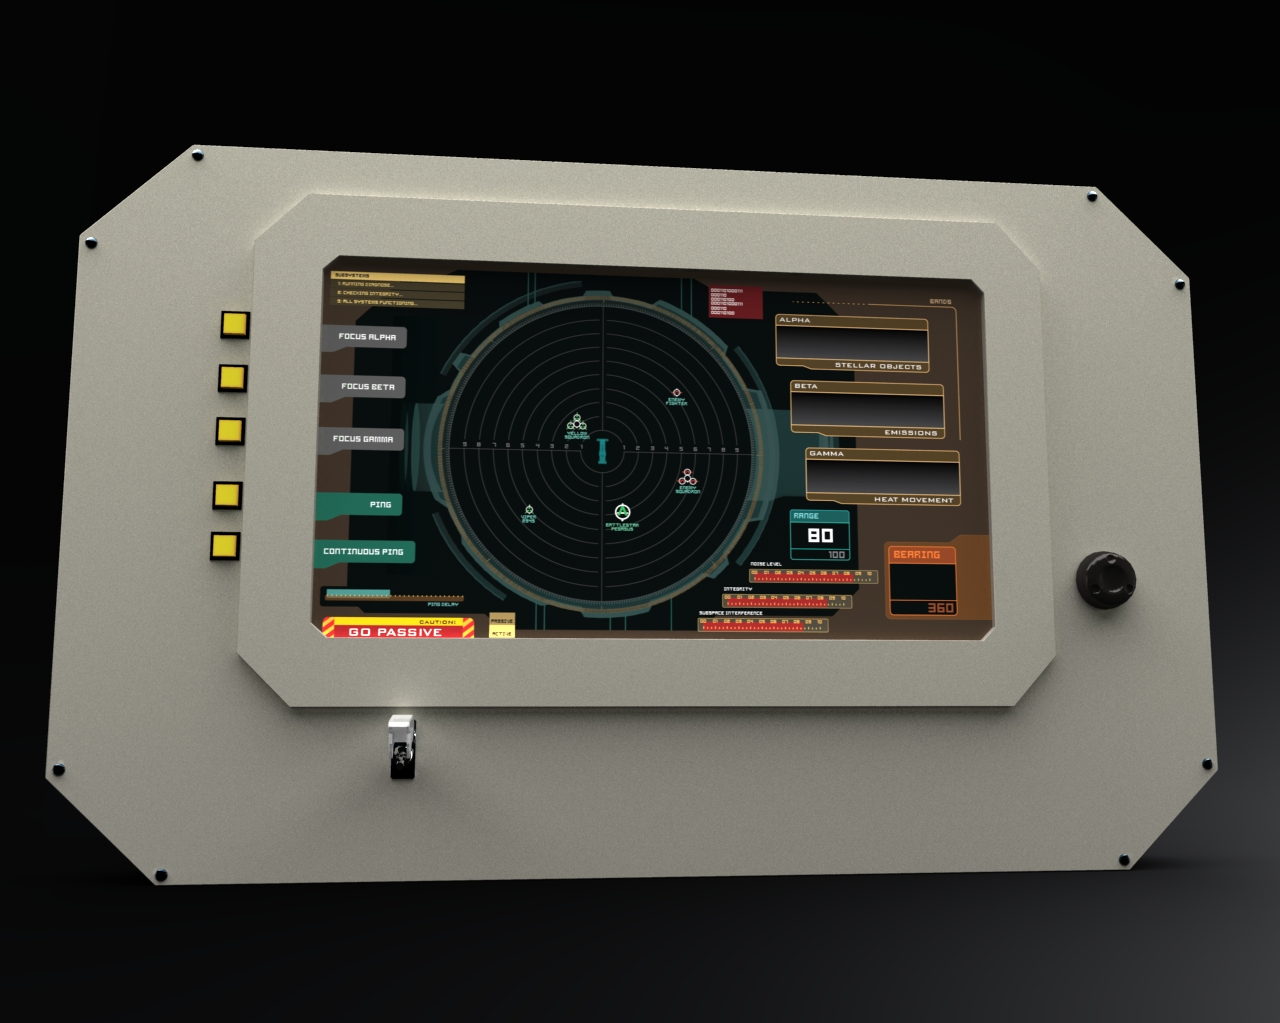
\includegraphics[width=0.4\textwidth]{img/Dradis.jpg}\hfill
  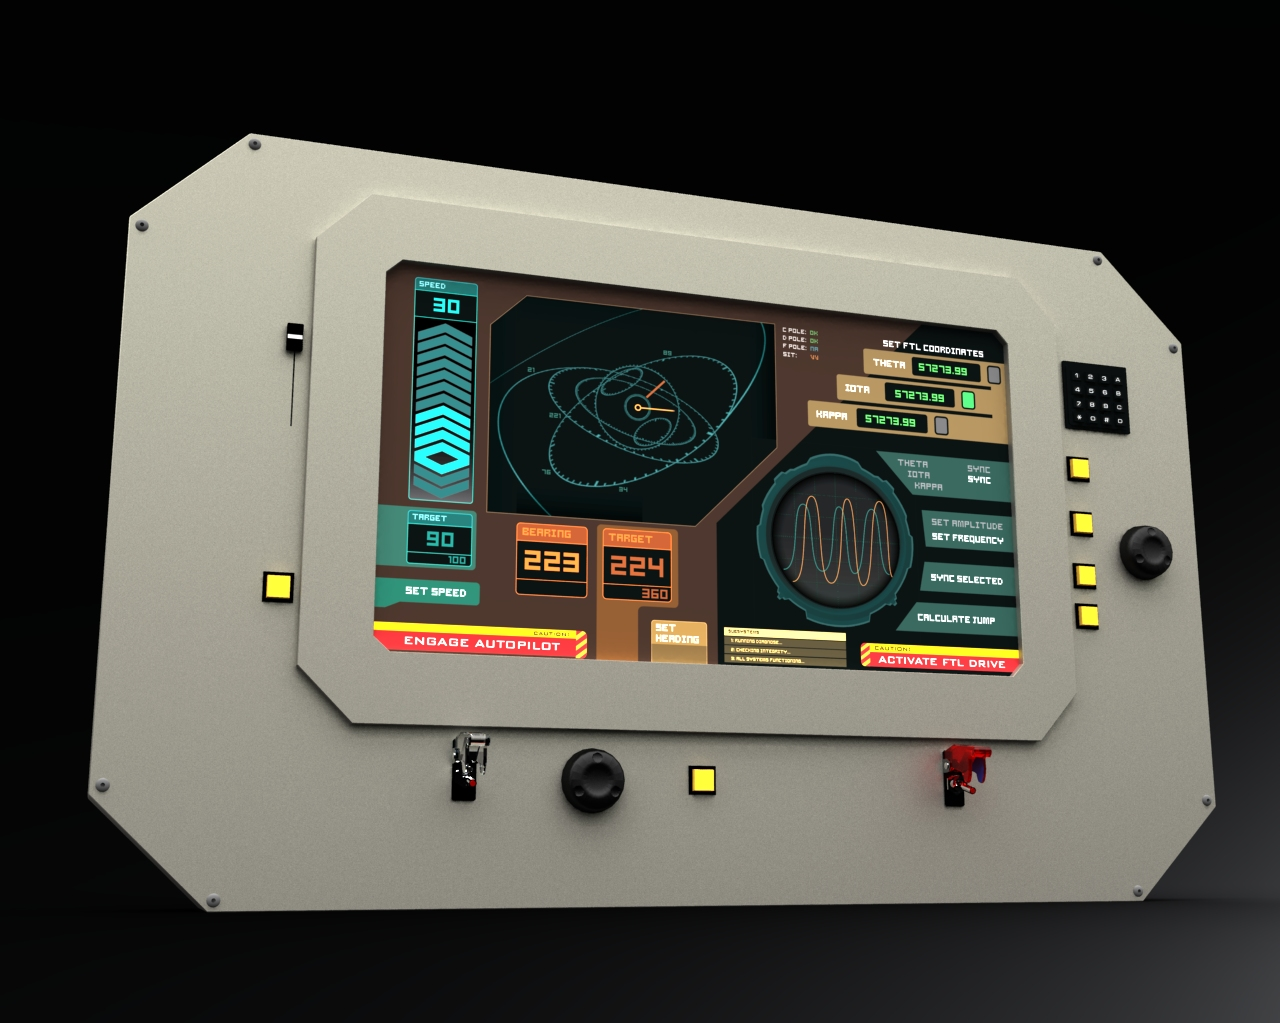
\includegraphics[width=0.4\textwidth]{img/Helm.jpg}
  \caption{The control panels for the active scanner and the FTL drive.}
  \label{fig:dradis}
\end{figure}


\subsection{Ambient loops}
\label{sec:ambient-loops}

The game was designed with three ambient noise loops: one global, with the general soundscape of a space ship in action, and two localized loops with reactor sounds and the command bridge sounds. All these needed to be started as each game session started up, and we built a single trigger to create all of them:

\begin{listing}
\begin{verbatim}
Trigger "startup loops trigger" 
 (MatchEvent "sound.trigger.startup") 
 (Execute "bridge ambience loop" 
   (concatSS 
    (map 
     (\i -> Loop "136_bridgeambience" i 0 (10,10)) 
     [8,9,10,11])) :++
  Execute "reactor ambience loop" 
   (Loop "124_reactor_run" 12 0 (60,60)) :++
  Execute "sound of celestra loop" 
   (concatSS  
    (map 
     (\i -> Loop "103_soundofcelestra" i 0 (20,20)) 
     global))),
\end{verbatim}
\caption{Reactive trigger that launches the ambient sound loops at the
start of the game.}
\end{listing}

The bridge was controlled by stations 8--11, while the large sub-woofer system for the deafening noise of the reactor engines was sound station 12. 

In addition to these loops, one more looping sound was included. If a general alarm was sounded for some reason, the blaring siren sound sat in a loop construct.

\begin{listing}
\begin{verbatim}
Trigger "alarm trigger" 
 (MatchEvent "sound.trigger.alarm") 
 (Execute "alarm" 
  (concatSS 
   (map 
    (\i -> Loop "137_generalalarm" i 0 (50,50)) 
    global))),
\end{verbatim}
\caption{Reactive trigger that launches the general alarm siren sound
  as a loop.}
\end{listing}

\subsection{Attack-decay-sustain-release}
\label{sec:attack-decay-sustain}

A large family of the sounds used in the soundscape went through a sequence of sound files, with fades between them. First, one sound would start the sequence. Next, a loopable sound would keep the sequence running -- preferably of a length that could be determined by the game masters at will. Finally, a sound would finish the noise sequence, often indicating success or failure of the corresponding player action.

These were common enough and repetitive enough that we ended up building a specific function to generate them. In the \texttt{SoundSpec.hs} source file, we defined a function \texttt{attackLoopDecay} that generated a sequence of chained sound commands.

\begin{listing}
\begin{verbatim}
attackLoopDecay :: 
  Id -> -- ^ Slug to generate ids for this command set
  Id -> -- ^ atF: attack sound
  Loudness -> -- ^ atL: attack loudness
  Int -> -- ^ t: time before fadeover
  Id -> -- ^ lpF: loop sound
  Loudness -> -- ^ lpL: loop loudness
  [Int] -> -- ^ locs: location list
  [(FilterSpec, SoundCommand)] -> -- ^ opts: Options for phasing out
  SoundCommand
attackLoopDecay slug atF atL t lpF lpL locs opts = 
 Execute (slug ++ "attack") 
         (foldl (:+) NopS (map (\i -> Play atF i 0 atL) locs)) :++
 Execute (slug ++ "loop") 
         (foldl (:+) NopS (map (\i -> Play lpF i t (0,0)) locs)) :++
 Execute (slug ++ "xfade") 
         ((FadeId (slug ++ "attack") t (t+100) (0,0)) :+
          (FadeId (slug ++ "loop") t (t+100) lpL)) :++
 (foldl (:++) Nop 
  (map 
   (\ (i,(fs,sc)) -> 
     Trigger (slug++"trigger"++(show i)) 
             fs 
             (sc :++ 
              foldl (:++) 
                    (Execute (slug++"stop") 
                             (StopId (slug ++ "loop") 0))
                    (map 
                      (\j -> Delete (slug ++ "trigger" ++ show j))
                      ([1..length opts]))
   ))
  (zip [1..] opts)))
\end{verbatim}
\caption{The \texttt{attackLoopDecay} utility function}
\end{listing}

First, we execute the sound \texttt{atF} at loudness \texttt{atL} and
at all the locations in \texttt{locs}. Next, we launch the loop after
a delay of \texttt{t} and at loudness 0. We launch our cross-fade
sequence at \texttt{t+100}ms going from the attack sound to the loop
sound. Finally, we generate a family of triggers for the possible
phasing out options. Each such trigger has a numbered identifier, and
contains both the required action for the phasing out option in
\texttt{sc}, as well as commands to stop playing the loop and to clean
out all the alternative phase out options.

With this utility function in place, we are able to construct sound
sequences for potentially failing player-initiated events -- such as
using the Faster-Than-Light jump drive.

\begin{listing}
\begin{verbatim}
Trigger "ftl jump trigger" 
 (MatchEvent "space.console.ftl_jump_started") 
 ((Execute "ftl jump voice" 
   (concatSS 
    (map 
     (\i -> Play "314_initiating_FTL" i 0 (80,80)) 
     global))) :++ 
  (attackLoopDecay "ftl jump " 
     "117_FTLspinningup" (80,80) 150 
     "123_FTLspinupcomplete" (80,80) 
     global 
     [(MatchEvent "space.console.ftl_jump_completed", 
       Execute "ftl jump completed" 
        (concatSS 
         (map 
          (\i -> Play "119_FTLjump" i 0 (80,80) :+ 
                 Play "318_FTLcomplete" i 9000 (100,100)) 
          global))),
      (MatchEvent "space.console.ftl_jump_failed", 
       Execute "ftl jump failed" 
        (concatSS 
         (map 
          (\i -> Play "118_FTLfail" i 0 (80,80) :+ 
                 Play "317_FTLmalfunction" i 4000 (100,100)) 
          global)))]))
\end{verbatim}
\caption{Reactive trigger event to launch the FTL jump sound sequence,
with two options for sequence finish: one for success, one for failure.}
\end{listing}

When the FTL command console initiates a jump sequence, the
\texttt{AMQP} message \texttt{space.console.ftl\_jump\_started'} is
issued. This launches a sound system reaction that first triggers the
synthetic voice announcing ship-wide that FTL has been initiated, by
playing \texttt{314\_initiating\_FTL} everywhere.

Next, we call the \texttt{attackLoopDecay} construct to generate the
sounds for spinning up and running the FTL engine. The related sounds
are named \texttt{ftl jump attack}, \texttt{ftl jump loop},
\texttt{ftl jump xfade}, \texttt{ftl jump trigger 1}  and \texttt{ftl
  jump trigger 2}.

The two triggerable end sounds are triggered with the game master
generated \texttt{space.console.ftl\_jump\_completed} and
\texttt{space.console.ftl\_jump\_failed} messages respectively, and
play a sound and a synthetic voice message corresponding to the result.

\subsection{Countdown}
\label{sec:countdown}

Never actually used in game, we also prepared a way to generate a
synthetic voice counting down. We had pre-recorded numbers that could
be concatenated, but needed to string them together programmatically.

To do this, we adapted the game engine to send out timing signals over
\texttt{AMQP} every second, every 10 seconds, every 30 seconds and
every minute. With these, we could construct functions that generated
triggers listening to these timing signals and generating appropriate
sound commands for the countdown sequence. They were all variants of
the same fundamental structure, illustrated in Listing~\ref{lst:minutes}

\begin{listing}
\begin{verbatim}
minutes n = 
 Declare 
  ("countdown " ++ show n ++ "m0s")
  (Trigger "countdown"
   (MatchEvent "sound.heartbeat.minute")
   (Execute "countdown" 
    (concatSS 
     (map 
      (\i -> 
       Play "Countdown/T minus" i 0 (100,100) :+
       Play ("Countdown/" ++ show n) i 1000 (100,100) :+
       Play "Countdown/Minutes and counting" i 2000 (100,100)) global)) :++
    Call ("countdown " ++ show (n-1) ++ "m0s")))
\end{verbatim}
\caption{Function to parametrically define a trigger event to launch a
minute-by-minute count down sound sequence.}
\label{lst:minutes}
\end{listing}

Calling \texttt{minutes 3} would store a \texttt{SoundCommand} named
\texttt{countdown 3m0s} that generated a trigger waiting for the next
\texttt{sound.heartbeat.minute} event and then playing a synthetic
voice saying \textit{Countdown T minus three minutes and
  counting}. Finally, the event would look up and call the stored
\texttt{SoundCommand} named \texttt{countdown 2m0s}.

For the last 15 minutes, the countdown would drop down to counting
every 30 seconds; for the last minute, it would count every 10 seconds, for
the last 10 seconds, it would count every second.

Access to these chains of callable commands was given to the game
masters by generating triggers through versions of the trigger given
in Listing~\ref{lst:minutetrigger}.

\begin{listing}
\begin{verbatim}
minuteTrigger n = 
 Trigger 
  ("countdown trigger " ++ show n ++ "m0s") 
  (MatchEvent ("sound.trigger.countdown." ++ show n ++ "m0s")) 
  (Call ("countdown " ++ show n ++ "m0s"))
\end{verbatim}
\caption{Game master callable triggers to launch the countdown
  sequence from a parametrizable starting time.}
\label{lst:minutetrigger}
\end{listing}

When an \texttt{AMQP} message of the form
\texttt{sound.trigger.countdown.25m0s} arrives, the trigger generated
by a call to \texttt{minuteTrigger 25} is activated. This trigger
looks up and calls the stored \texttt{SoundCommand} named
\texttt{countdown 25m0s}, which hooks into the chains of
\texttt{SoundCommand}s described above.

%%% Local Variables: 
%%% mode: latex
%%% TeX-engine: default
%%% TeX-master: "tmr"
%%% End: 
